This article is likely to be useful for those who are going to sit the Senior Maths Challenge, and who then hope to sit the British Mathematical Olympiad as a result; however, other members of the school may do this later in their school career, and so should consider reading on anyway.

Sometimes one is not able to easily solve an Olympiad geometry question through the usual method, or is unable to work out how to do so. At such times, some try to use Cartesian coördinates to reduce such problems to mere algebra. This barely ever works. However, sometimes other coördinate systems do the trick. This week, we shall be looking at areal coördinates, which work particularly well on geometry questions which centre on a triangle.

\begin{figure}
\centering
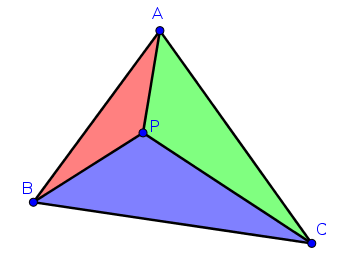
\includegraphics{areals.png}
\caption{A point \(P\) inside triangle \(ABC\)}
\end{figure}

In areal coördinates, we say that a point \(P\) inside the triangle has coördinates \(x,y,z\) with respect to triangle \(ABC\) if \[|PBC|:|PCA|:|PAB|=x:y:z\]
(where \(|XYZ|\) denotes the area of triangle \(XYZ\).

\begin{figure}
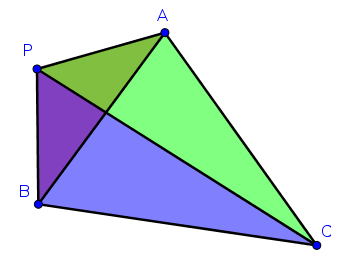
\includegraphics{areals2.png}
\caption{A point \(P\) outside triangle \(ABC\)}
\end{figure}

We extend this to points outside the triangle by directing the areas; that is to say, in such a configuration as Figure 2, \(PAB\) is negative, as \(P\) is on a different side of \(AB\) to the triangle; however, \(PBC\) is positive, because although \(P\) is outside the triangle, it is on the same side of \(BC\) as the triangle.

The best way to explain how one uses areal coördinates is to give an example; I have included a somewhat lengthy one, which explains and gives reasons for a variety of interesting and useful properties of areal coördinates.

\subsection{Question}

Let \(ABC\) be an acute-angled triangle; let the altitudes of the triangle (i.e. the perpendiculars from points of the triangle to the opposite sides) be \(AD\), \(BE\), \(CF\), such that \(D, E, F\) lie on \(BC, AC, AB\) respectively; let the angle bisectors of the triangle be \(AP, BQ, CR\) such that \(P, Q, R\) lie on \(BC, AC, AB\) respectively; let the incentre of the triangle (the centre of the circle inside the triangle that is tangent to all three sides (which we call the incircle))) be \(I\); let the circumcentre of the triangle (the centre of the circle that passes through all three points of the triangle (which we call the circumcircle)) be \(O\). Prove that \(D, I, E\) lie on a single straight line if and only if \(P, O, Q\) also lie on a single straight line.

\subsection{Solution}

Henceforth \(a=|BC|\), \(b=|AC|\), \(c=|AB|\), angles \(A,B,C\) are \(\angle{}CAB\), \(\angle{}ABC\), and \(\angle{}BCA\) respectively, \(r\) denotes the radius of the incircle, and \(R\) denotes the radius of the circumcircle.

Note that henceforth \((x:y:z)\) denotes the point \((x,y,z)\) in areal coördinates of triangle \(ABC\).

Firstly, it should be noted that where point \(X=(x:y:z)\), \(AX\) meets \(BC\) at \(Y=(0:y:z)\), as the area of \(YBC\) is naturally 0 and the ratios of the areas of \(YBA\) and \(YCA\) depend solely on the perpendicular distances of \(B\) and \(C\) from \(AY\) (by using the formula \(\frac{\textrm{base}\times{}\textrm{height}}{2}\) with \(AY\) as the base), which are the same as those from \(AX\). By similar logic, \(BX\) meets \(AC\) at \((x:0:z)\).

The incentre, \(I\), is \((a:b:c)\) as it is perpendicularly equidistant from all three sides of the triangle, so the areas of \(AIB, AIC, BIC\) are proportional to \(AB, AC, BC\) (as the heights of the triangles are all the radius of the incircle), and so \(|IBC|:|IAC|:|IAB|=\frac{ra}{2}:\frac{rb}{2}:\frac{rc}{2}=a:b:c\). Then, by our earlier findings, \(P\) and \(Q\) which lie on angle bisectors passing through \(I\), are respectively \((0:b:c)\) and \((a:0:c)\).

Now, using the formula for the area of a triangle being \(\frac{ab\sin(C)}{2}\), the circumcentre, \(O\), is \((\sin(\angle{}BOC)\frac{r^2}{2}:\sin(\angle{}AOC)\frac{r^2}{2}:\sin(\angle{}AOB)\frac{r^2}{2})\) \(=(\sin(\angle{}BOC):\sin(\angle{}AOC):\sin(\angle{}AOB))\). By the \say{angle at the centre of the circle is twice that at the circumference} theorem, \(O=(\sin(2A):\sin(2B):\sin(2C))\).

To find \(D\) and \(E\), we must first find the orthocentre, \(H\). Using triangle \(ABD\), \(BD=c\cos(B)\); using \(\angle{}BEC=90^{\circ}\), \(\angle{}EBC=90^{\circ}-C\) and so \(DH=BD\tan(\angle{}EBC)=c\cos(B)\frac{\sin(90^{\circ}-C)}{\cos(90^{\circ}-C)}=c\cos(B)\frac{\cos(C)}{\sin(C)}\). By the sine rule, this equals \(2R\cos(B)\cos(C)\), and so the area of triangle \(HBC\) is \(aR\cos(B)\cos(C)\). By similar logic, the areal coördinates of the orthocentre are
\[a\cos(B)\cos(C)R:\cos(A)b\cos(C)R:\cos(A)\cos(B)cR\]
Dividing by \(R^2\), we get
\[\begin{split}
\sin(A)\cos(B)\cos(C):\\
\cos(A)\sin(B)\cos(C):\\
\cos(A)\cos(B)\sin(C)
\end{split}\]
Dividing again by \(\cos(A)\cos(B)\cos(C)\), we find
\[H=(\tan(A):\tan(B):\tan(C))\]
from which we then easily find that \(D=(0:\tan(B):\tan(C))\) and \(E=(\tan(A):0:\tan(C))\). We now have all the points we are going to use.

Using areal coördinates, it is known and accepted that \((a:b:c)\), \((d:e:f)\), and \((g:h:i)\) are colinear if and only if
\[
\begin{vmatrix}
a&b&c\\
d&e&f
\\g&h&i
\end{vmatrix}=0
\]

For the readers who are as yet unaware of matrix determinants, here is a definition of this particular size thereof.

\[
\begin{vmatrix}
a&b&c\\
d&e&f
\\g&h&i
\end{vmatrix}=aei+bfg+cdh-ceg-bdi-afh
\]

Readers are however encouraged to look up the full definition.

This means the original statement can be, if not simplified, rephrased as proving that

\[
\begin{split}
\begin{vmatrix}
a&b&c\\
0&\tan(B)&\tan(C)
\\\tan(A)&0&\tan(C)
\end{vmatrix}
=0
\iff{}
\\
\begin{vmatrix}
\sin(2A)&\sin(2B)&\sin(2C)\\
0&b&c\\
a&0&c
\end{vmatrix}
=0
\end{split}{}
\]

Multiplying out the determinants and moving the negative terms onto the right hand side, we find that this statement is equivalent to
\[a\tan(B)\tan(C)+\tan(A)b\tan(C)=\tan(A)\tan(B)c\]\[\iff{}\]\[\sin(2A)bc+a\sin(2B)c=ab\sin(2C)
\]
Dividing the first equation by \(\tan(A)\tan(B)\tan(C)\) and the second by \(abc\) we find the statement is equivalent to
\[
\begin{split}
\frac{a}{\tan(A)}+\frac{b}{\tan(B)}=\frac{c}{\tan(C)}
\iff \\
\frac{\sin(2A)}{a}+\frac{\sin(2B)}{b}=\frac{\sin(2C)}{c}
\end{split}
\]
From \(\sin(A+B)=\sin(A)\cos(B)+\cos(A)\sin(B)\), it is clear that \(\sin(2A)=2\sin(A)\cos(B)\); so we can now use that to simplify the second equation, and expand \(\tan(A)\) into \(\frac{\sin(A)}{\cos(A)}\) in the first, giving us
\[
\frac{a\cos(A)}{\sin(A)}+\frac{b\cos(B)}{\sin(B)}=\frac{c\cos(C)}{\sin(C)}\]
\[\iff\]
\[\frac{\sin(A)\cos(A)}{a}+\frac{\sin(B)\cos(B)}{b}=\frac{\sin(C)\cos(C)}{c}
\]
This is clearly equivalent to
\[\begin{split}
2R\cos(A)+2R\cos(B)=2R\cos(C)
\iff\\
\frac{cos(A)}{2R}+\frac{cos(B)}{2R}=\frac{cos(C)}{2R}
\end{split}
\]
Then, dividing the first equation by \(2R\) and multiplying the second by it, we have
\[\begin{split}
\cos(A)+\cos(B)=\cos(C)
\iff\\
\cos(A)+\cos(B)=\cos(C)
\end{split}
\]
which is clearly true, and as it is equivalent to the original statement, the original statement must also be true. \(\blacksquare{}\)
